\section{小さな VLM の二段階の学習}
\label{sec_vlm}
\subsection{分類器の構成}
お題画像とボケの両方を入力とする生徒として，1〜8B の VLM を分類器にした．
VLM に，お題画像と「大喜利サイト「ボケて」のお題画像（形式：$ \cdot $）に投稿されたボケ：「$ \cdot $」」という文を入力し，言語モデルの最終層の，入力の最後のトークンの隠れ状態 $ {\mathbf h} \in {\mathbb R}^{H} $ を取り出す．
発話の型の確率 $ {\mathbf p} \in {\mathbb R}^{6} $ と画像外の知識の確率 $ q $ を，(\ref{eq_heads})で求める．

\begin{align}
    {\mathbf p} &= {\rm softmax} ( {\mathbf W}_{\rm v} {\mathbf h} + {\mathbf b}_{\rm v} ) \nonumber \\
    q &= \sigma ( {\mathbf w}_{\rm o}^{\top} {\mathbf h} + b_{\rm o} )
    \label{eq_heads}
\end{align}

\noindent
ここで $ {\mathbf W}_{\rm v} \in {\mathbb R}^{6 \times H} $，$ {\mathbf b}_{\rm v} \in {\mathbb R}^{6} $，$ {\mathbf w}_{\rm o} \in {\mathbb R}^{H} $，$ b_{\rm o} \in {\mathbb R} $ は出力層のパラメータ，$ \sigma $ はシグモイド関数，$ H $ は隠れ状態の次元数である．
生成を行わず1回の順伝播で判定するため，VLM に回答を生成させる場合より速い．
VLM の全ての線形層にランク16の LoRA\cite{ref_lora}を付けて学習した．
お題画像は長辺448画素以下に縮小し，タイル分割を止めて画像のトークン数を200〜300程度にそろえた．

損失は，発話の型の正解 $ y $ と画像外の知識の正解 $ t \in \{0, 1\} $ に対し，(\ref{eq_loss})とした．

\begin{equation}
    {\mathcal L} = - \alpha_{y} \log p_{y} - \lambda \left\{ \beta \, t \log q + (1 - t) \log (1 - q) \right\}
    \label{eq_loss}
\end{equation}

\noindent
ここで $ \alpha_{y} $ は学習データでのクラス $ y $ の出現率の逆数の平方根に比例する重み，$ \beta $ は負例と正例の件数の比，$ \lambda $ は画像外の知識の損失の重み（\ref{sec_outside}章を除き $ \lambda = 1 $）である．
最適化には AdamW\cite{ref_adamw}を用い，LoRA の学習率を $ 10^{-4} $，出力層をその10倍とし，最初の5\%のステップで線形に増やした後に余弦関数で減衰させた．

\subsection{学習の手順}
学習は次の二段階で行った．
\begin{enumerate}
    \item 段階1：教師（32B，one\_kt\_cap）のラベル34,634件で，バッチサイズ16で1〜2エポック学習する．教師ラベルの1割を検証用に取り分けた．
    \item 段階2：段階1の重みから，学習用の目視ラベル931件で，バッチサイズ8，学習率 $ 5 \times 10^{-5} $ で4エポック微調整し，調整用データで最良のエポックを選ぶ．
\end{enumerate}
学習用の目視ラベル931件は，教師ラベルの集合（検証データのお題を含まない）から，お題1件につき1件まで抽出した．
半数は無作為に選び，残りは教師ラベルで少ない型（心の声，ツッコミ，状況の説明，名付け・見立て）と画像外の知識が「はい」のボケを多めに選んだ．
内訳は，セリフ248件，回答206件，状況の説明156件，名付け・見立て152件，心の声109件，ツッコミ60件であり，画像外の知識が「はい」は26\%であった．
この931件で教師ラベルと目視ラベルを比べると，6区分のマクロ F1 は0.65（ツッコミ0.33，状況の説明0.51），画像外の知識の F1 は0.63であり，教師ラベルには大きな誤りが含まれていた．

比較のため，指示だけで判定させる方法（ゼロショット）と，段階1を行わず目視ラベルだけで8エポック学習する方法も評価した．
ゼロショットでは，vLLM で one\_kt\_cap の指示を与えて JSON を生成させた．

\subsection{結果}
表\ref{tab_zeroshot}にゼロショットの結果を，表\ref{tab_vlm}に微調整の結果を，図\ref{fig_progress}に段階ごとの最終評価用データでの F1 を示す．

\begin{table}[t]
    \centering
    \caption{ゼロショットの比較（合意ラベル）．速度は vLLM で620件を一括で生成したときの1秒あたりの件数，形式は JSON を読み取れた割合．（推）は推論の後に回答する Thinking モデル．}
    \label{tab_zeroshot}
    \footnotesize
    \setlength{\tabcolsep}{1.8pt}
    \begin{tabular}{@{}lcccccc@{}}
        \toprule
        & \multicolumn{2}{c}{6区分} & 3区分 & 画像外 & & \\
        モデル & dev & test & test & test & 速度 & 形式 \\
        \midrule
        Qwen3-VL-2B & 0.28 & 0.28 & 0.54 & 0.44 & 11.7 & 1.00 \\
        Qwen3-VL-4B & 0.44 & 0.42 & 0.74 & 0.39 & 15.2 & 1.00 \\
        Qwen3-VL-8B & 0.44 & 0.41 & 0.71 & 0.56 & 11.9 & 1.00 \\
        InternVL3.5-1B & 0.30 & 0.30 & 0.56 & 0.00 & 13.5 & 1.00 \\
        InternVL3.5-2B & 0.25 & 0.29 & 0.56 & 0.00 & 11.5 & 1.00 \\
        InternVL3.5-4B & 0.30 & 0.32 & 0.67 & 0.00 & 7.3 & 1.00 \\
        LFM2-VL-1.6B & 0.29 & 0.28 & 0.64 & 0.00 & 24.8 & 0.99 \\
        LFM2-VL-3B & 0.30 & 0.26 & 0.56 & 0.07 & 19.0 & 1.00 \\
        SmolVLM2-2.2B & 0.25 & 0.26 & 0.58 & 0.00 & 5.1 & 1.00 \\
        Gemma 3 4B & 0.31 & 0.32 & 0.58 & 0.57 & 8.3 & 1.00 \\
        Qwen3-VL-30B-A3B（推） & 0.45 & 0.48 & 0.72 & 0.50 & 0.7 & 0.56 \\
        Qwen3-VL-32B（推） & \textbf{0.50} & \textbf{0.52} & \textbf{0.79} & \textbf{0.61} & 0.3 & 0.77 \\
        \bottomrule
    \end{tabular}
\end{table}

\begin{table}[t]
    \centering
    \caption{小さな VLM の微調整の比較（合意ラベル．dev は調整用，test は最終評価用）．速度は前処理を含む1秒あたりの件数（分類器の推論，バッチ32）．}
    \label{tab_vlm}
    \footnotesize
    \setlength{\tabcolsep}{3pt}
    \begin{tabular}{@{}lccccc@{}}
        \toprule
        & \multicolumn{2}{c}{6区分} & 3区分 & 画像外 & \\
        方法 & dev & test & test & test & 速度 \\
        \midrule
        \multicolumn{6}{@{}l}{段階1のみ（教師ラベル）} \\
        \quad Qwen3-VL-4B & 0.61 & 0.55 & 0.79 & 0.70 & 33 \\
        \quad InternVL3.5-2B & 0.58 & 0.57 & 0.79 & 0.66 & 46 \\
        \multicolumn{6}{@{}l}{目視ラベルのみ} \\
        \quad Qwen3-VL-4B & 0.69 & 0.67 & 0.84 & 0.55 & 33 \\
        \quad Qwen3-VL-2B & 0.69 & 0.71 & 0.86 & 0.55 & --- \\
        \multicolumn{6}{@{}l}{段階1＋段階2} \\
        \quad InternVL3.5-1B & 0.71 & 0.69 & 0.85 & 0.61 & --- \\
        \quad InternVL3.5-2B & \textbf{0.77} & 0.71 & 0.85 & 0.64 & 46 \\
        \quad InternVL3.5-4B & 0.72 & 0.71 & 0.85 & 0.67 & --- \\
        \quad Qwen3-VL-2B & 0.69 & 0.65 & 0.84 & 0.62 & --- \\
        \quad Qwen3-VL-4B & 0.76 & 0.71 & 0.86 & 0.69 & 33 \\
        \quad LFM2-VL-1.6B & 0.71 & 0.64 & 0.85 & 0.64 & --- \\
        \bottomrule
    \end{tabular}
\end{table}

\begin{figure}[t]
    \centering
    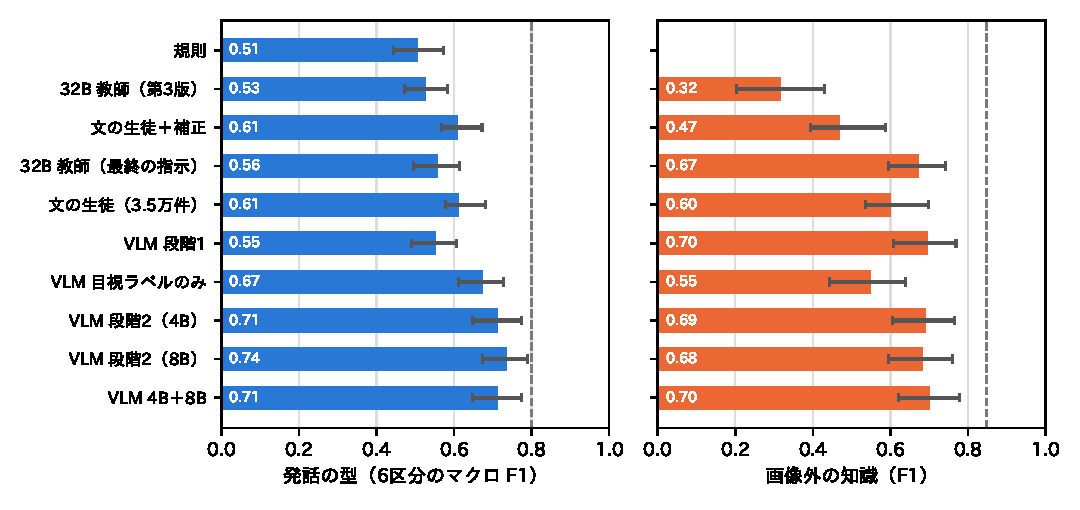
\includegraphics[width=\linewidth]{figures/fig_progress.pdf}
    \caption{主な段階の方法の最終評価用データ（312件）での F1 と95\%信頼区間．破線は目視ラベルの再現性（表\ref{tab_reliability}）．規則は画像外の知識を判定しない．}
    \label{fig_progress}
\end{figure}

ゼロショットでは，小さな VLM は指示だけでは判定できなかった．
6区分は最良の Qwen3-VL-4B でも0.42であり，InternVL3.5，LFM2-VL，SmolVLM2 は画像外の知識をほぼ全て「いいえ」とした．
推論を行う 32B の Thinking モデルも，6区分0.52，画像外の知識0.61で，教師（Instruct）を上回らなかった．
推論の後に JSON を書き終えない出力が23\%あり，速度は教師の1/10以下であった．

段階1だけの VLM は，画像外の知識で教師と同等以上（Qwen3-VL-4B で0.70）となったが，6区分は教師と同程度の0.55〜0.57であった．
教師ラベルを再現するところまでは学べるが，教師の誤りも再現したと考えられる．
段階2の微調整により，6区分は全てのモデルで段階1より0.12〜0.16上がり，0.64〜0.71となった．
目視ラベルだけで学習した場合，6区分は同程度の0.67〜0.71であったが，画像外の知識は0.55で，段階1を経た場合（0.69）より大きく低かった．
すなわち，画像外の知識は大量の教師ラベルから，6区分の境界は少量だが正確な目視ラベルから学んでいると考えられる．

段階2の後のクラスごとの F1 は，セリフ0.83，回答0.91，状況の説明0.76〜0.78，名付け・見立て0.74〜0.77に対し，心の声0.58〜0.64，ツッコミ0.36〜0.45であった．
表\ref{tab_per_class}に，クラスごとの F1 を目視ラベルの再現性と比べて示す．
目視ラベルの再現性でも低いツッコミと心の声が，マクロ F1 を下げている．

\begin{table}[t]
    \centering
    \caption{発話の型のクラスごとの F1（最終評価用）．再現性は元の目視ラベルと付け直したラベルの一致（620件）．括弧内は最終評価用の件数．文の生徒は seed 0 の値．}
    \label{tab_per_class}
    \footnotesize
    \setlength{\tabcolsep}{2.5pt}
    \begin{tabular}{@{}lcccccc@{}}
        \toprule
        方法 & S (110) & M (31) & T (14) & N (42) & L (43) & A (72) \\
        \midrule
        教師 32B & 0.70 & 0.44 & 0.17 & 0.54 & 0.58 & 0.91 \\
        文の生徒 & 0.74 & 0.54 & 0.23 & 0.74 & 0.62 & 0.91 \\
        InternVL3.5-2B & 0.83 & 0.64 & 0.36 & 0.78 & 0.77 & 0.91 \\
        Qwen3-VL-4B & 0.83 & 0.58 & 0.45 & 0.76 & 0.74 & 0.91 \\
        Qwen3-VL-8B & 0.85 & 0.65 & 0.43 & 0.77 & 0.81 & 0.90 \\
        \midrule
        再現性 & 0.89 & 0.75 & 0.55 & 0.85 & 0.81 & 0.94 \\
        \bottomrule
    \end{tabular}
\end{table}
最終評価用データでの6区分の95\%信頼区間は，InternVL3.5-2B で0.65〜0.77，Qwen3-VL-4B で0.65〜0.77であった．

\subsection{目視ラベルの量}
目視ラベルの量と精度の関係を調べるため，Qwen3-VL-4B の段階2を，931件の25\%と50\%で行った．
図\ref{fig_learning_curve}に結果を示す．

\begin{figure}[t]
    \centering
    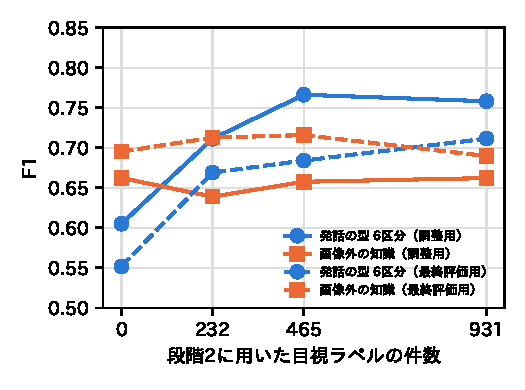
\includegraphics[width=0.95\linewidth]{figures/fig_learning_curve.pdf}
    \caption{段階2に用いた目視ラベルの件数と F1（Qwen3-VL-4B）．0件は段階1のみである．}
    \label{fig_learning_curve}
\end{figure}

最終評価用データの6区分は，232件で0.67，465件で0.68，931件で0.71と，目視ラベルを倍にするごとに0.015〜0.03程度伸びた．
一方，画像外の知識は0.69〜0.72で，目視ラベルの量によらずほぼ一定であった．
931件に検証データの半分（約310件）を加えて残りの半分を予測する2分割の実験でも，6区分は最終評価用で0.71と変わらなかった．
6区分の伸びが続くとしても，0.8に近づけるには数千件以上の目視ラベルが必要と見込まれる．
ただし，これは観測した点からの外挿であり，確かめていない．
